\documentclass[a4paper,10pt]{article}
%%!TEX encoding = UTF-8 Unicode
\usepackage{graphicx}
\usepackage[spanish]{babel}
\usepackage[utf8]{inputenc}
\usepackage{listings}
\lstset{basicstyle=\footnotesize,
stringstyle=\ttfamily,
showstringspaces=false,
frameround=fttt}
\usepackage{anysize}
\marginsize{3.5cm}{3.5cm}{2cm}{2cm}
%bordes en header y footer
\usepackage{fancyhdr}
\chead{TP N$^{\circ}$ 0 - Infraestructura básica}
\lhead{}
\rhead{}
\lfoot{66.20 - Organización de Computadoras}
\cfoot{}
\rfoot{\thepage}
\renewcommand{\headrulewidth}{0.35pt}
\renewcommand{\footrulewidth}{0.35pt}
\textheight 630pt
\topmargin 0pt
\pagestyle{fancy}
%%%%%%%%%%

\title{		\textbf{TRABAJO PRACTICO N$^{\circ}$ 0}\\ \textbf{Infraestructura básica}}

\author{	
	    Ezequiel Paez, \textit{Padrón Nro. }                     \\
            \texttt{  }                                            \\[2.5ex]
            Juan Manuel Gonzales, \textit{Padrón Nro. }                     \\
            \texttt{  }                                              \\[2.5ex]
            Osiris Argüello, \textit{Padrón Nro. 83062}                     \\
            \texttt{ osirisarguello@yahoo.com.ar }                                              \\[2.5ex]
            \normalsize{1er. Cuatrimestre de 2012}                                      \\
            \normalsize{66.20 Organización de Computadoras - Curso 02}  \\
            \normalsize{Facultad de Ingeniería, Universidad de Buenos Aires}            \\
       }
\date{}


\begin{document}

\maketitle
\thispagestyle{empty}   
\newpage
\setcounter{page}{5} 
\tableofcontents
\newpage

\section{Resumen}
En el presente trabajo práctico, se deben implementar en un programa en lenguaje C dos algoritmos de ordenamiento: Mergesort y Selection sort.
Una vez implementados, procederemos a realizar mediciones para evaluar las posibilidades de mejora y el desempeño relativo entre ambas implementaciones, utilizando los programas time y gprof.


\section{Diseño e Implementación}
El diseño de la aplicación se realizó pensando en varias <<capas>>. Una capa es encargada de analizar y validar opciones de ejecución, otra capa, la encargada de realizar las operaciones principales de conversión y otras más pequeñas encargadas de emitir mensajes de error o información de ayuda en pantalla para el usuario.\\

Dado que la aplicación puede tomar parámetros variables de ejecución o adoptar valores por defecto, se realizó un análisis completo de todas las opciones que un usuario puede ingresar, aceptando aquellas que fueren válidas y rechazando las que no, con el consiguiente mensaje de error que el usuario visualizará en pantalla.\\

La aplicación fue implementada en lenguaje ANSI C, es decir que está garantizada la compilación exitosa ante la utilización de la opción \textit{-ansi}.\\

La siguiente capa importante, es la capa de los algoritmos de ordenamiento. Se desarrollaron dos algoritmos de ordenamiento: \textit{mergesort} y \textit{selectionsort}. \\

La implementación para ambos algoritmos básicamente consta de procesos similares, ligeramente diferenciados en el punto en que se invoca una función ANSI C distinta de acuerdo al tipo de ordenamiento que se esté realizando. Como primer paso del algoritmo, se abre el \textit{stream} de entrada de datos que es especificado por el usuario. De no resultar satisfactoria esta operación, ya sea porque el archivo no existe o se produjere un fallo en el disco en el momento de la apertura, se retorna de inmediato el correspondiente código de error.\\
Si el archivo es abierto satisfactoriamente se procede a leer su contenido, realizando el ordenamiento indicado por el usuario y el resultado de dicha operación es volcado al archivo de salida también especificado en los parámetros de ejecución.\\

Las principales funciones en nuestra implementación son las siguientes:

\subsection{procesar\_ordenamiento}
Este método se encarga de tomar los archivos de entrada y salida, abrirlos y luego ejecutar el método de ordenamiento correspondiente.
Por último devuelve el resultado en el archivo de salida indicado.

\subsection{mergeSort}
Este método toma el array de caracteres leido del archivo, lo divide en 2 partes e invoca recursivamente la funcion \textbf{mergeSort} sobre cada parte.
Como ultimo paso invoca a la funcion \textbf{merge} para fusionar ambas partes, ordenandolas.

\subsection{selectionSort}
Este método recorre el array de caracteres, buscando el menor caracter en cada iteración y ubicandolo al principio del array.

\section{Instrucciones de Compilación}

Si el objetivo es exclusivamente obtener el ejecutable y probar la aplicación, las instrucciones básicas para compilación mediante línea de comandos (situado en el directorio que contiene el archivo <<main.c>>) son:\\

\begin{center}
\textit{\$ gcc -o tp0 main.c}\\
\end{center}

Donde:
\begin{itemize}
\item -o: archivo de salida (en este caso, tp0).
\end{itemize}

Si en cambio, se desean visualizar todos los mensajes de advertencia, verificar problemas de acceso a memoria, depurar el código, optimizarlo, etc., las opciones de compilación pueden ser:\\

\begin{center}
\textit{\$ gcc -Wall -g -o tp0 main.c}\\
\end{center}

Donde:
\begin{itemize}
\item -Wall: permite que se visualicen todos los mensajes de advertencia, 
\item -g: permite realizar un seguimiento generando información de depuración. Por ejemplo, con algún \textit{<<profiler>>} como \textit{\textbf{gdb}},
\item -o: archivo de salida (en este caso, tp0)
\end{itemize}

Para generar el código assembler se utiliza:\\
\begin{center}
\textit{\$ gcc -Wall -O0 -S -mrnames main.c},
\end{center}

Donde:
\begin{itemize}
\item -O0: indica nivel cero de optimización,
\item -S: envía la instrucción de no ejecutar el linker luego de generar el código assembler en el archivo \textit{main.s},
\item -mrnames (solo para MIPS): indica al compilador que genere la salida utilizando nombre de registro en lugar de número de registro.
\end{itemize}

\newpage
\section{Corridas de Prueba}

\subsection{Corridas exitosas}

Mensaje de ayuda. Se obtiene utilizando los comandos -h o --help.\\

\begin{figure}[!htp]
  \centering
    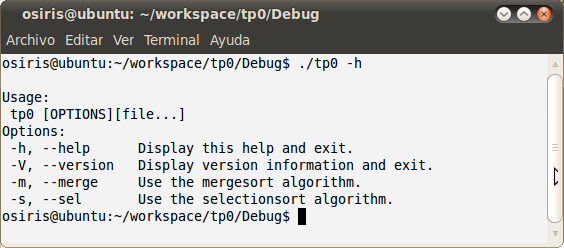
\includegraphics[width=9 cm]{tp0_opcion_help.png}
  \caption{Mensaje de ayuda}
  \label{Figura1}
\end{figure}

Versión del programa. Se obtiene utilizando los comandos -V o --version.\\

\begin{figure}[!htp]
	\centering
	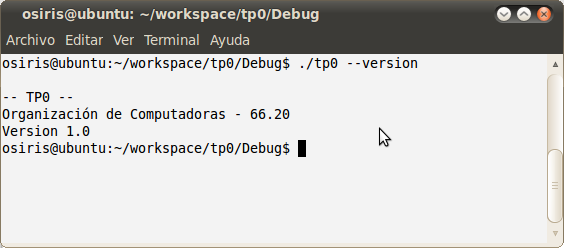
\includegraphics[width=9 cm]{tp0_opcion_version.png}
	\caption{Mensaje de versión del programa}
	\label{Figura2}
\end{figure}

Para esta corrida se eligió ordenar un archivo con dígitos y se prueban ambos métodos de ordenamiento. En el primer caso, al no pasar parámetro se está tomando por defecto el ordenamiento por mergesort. El resultado se muestra por pantalla.\\
\begin{figure}[!htp]
	\centering
	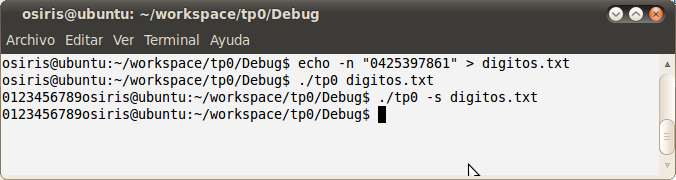
\includegraphics[width=10.5 cm]{tp0_corrida_exitosa_0.png}
	\caption{Ordenar digitos.txt}
	\label{Figura3}
\end{figure}

Para la siguiente corrida se eligió ordenar un archivo de caracteres con minusculas y mayusculas y se corren ambos métodos de ordenamiento. En el primer caso la entrada y la salida son por \textit{stdin} y \textit{stdout}. En el segundo ambos son archivos.\\
\begin{figure}[!htp]
	\centering
	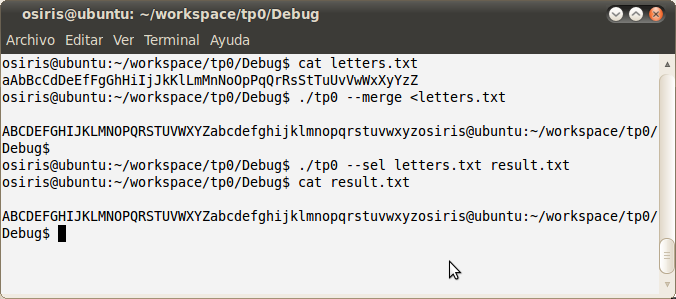
\includegraphics[width=10.5 cm]{tp0_corrida_exitosa_1.png}
	\caption{Ordenar letters.txt}
	\label{Figura4}
\end{figure}

En esta corrida se eligió ordenar un archivo con caracteres aleatorios.\\
\begin{figure}[!htp]
	\centering
	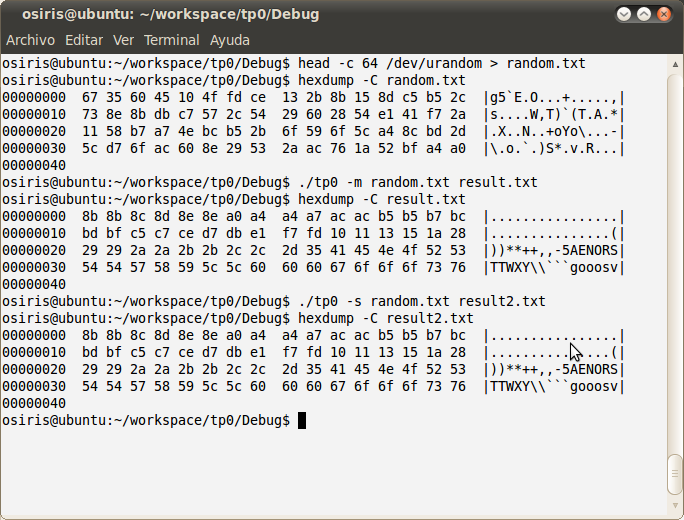
\includegraphics[width=10.5 cm]{tp0_corrida_exitosa_2.png}
	\caption{Ordenar random.txt}
	\label{Figura5}
\end{figure}



\newpage
\subsection{Mensajes de Error}
Las siguientes situaciones producen mensajes de error:\\

Si ocurre un fallo al abrir el file, se mostrará el mensaje de la figura junto con el nombre del file.\\

\begin{figure}[!htp]
	\centering
	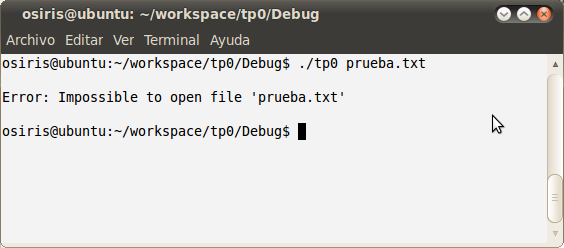
\includegraphics[width=8.5 cm]{tp0_error_openfile.png}
	\caption{Error al abrir el file}
	\label{Figura6}
\end{figure}

\newpage
Si al ejecutar se ingresan más parámetros de los que puede interpretar el programa, se mostrará el mensaje de la figura y seguido el menú de ayuda.\\
\begin{figure}[!htp]
	\centering
	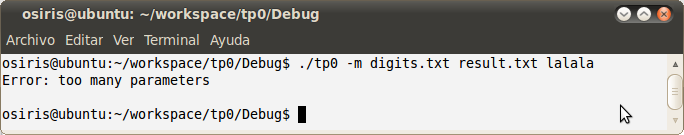
\includegraphics[height=2.1 cm]{tp0_error_2manyparam.png}
	\caption{Error debido a muchos parámetros}
	\label{Figura7}
\end{figure}

Si al ejecutar se ingresa algún parámetro inesperado por el programa, se mostrará el mensaje de la figura junto con el parámetro desconocido y el menú de ayuda.\\
\begin{figure}[!htp]
	\centering
	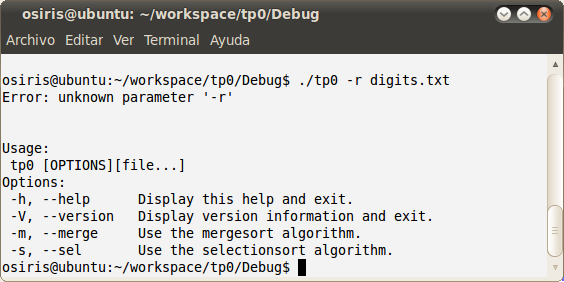
\includegraphics[height=4.3 cm]{tp0_error_unknownparam.png}
	\caption{Error por parámetro desconocido}
	\label{Figura8}
\end{figure}

\newpage
\section{Mediciones y Profiling}

\newpage
\section{Código fuente}
\subsection{Lenguaje C}

\noindent
\underline{main.c}

\begin{tiny}
\begin{lstlisting}
#include <stdio.h>
#include <string.h>
#include <stdlib.h>

void PrintHelp();
void PrintVersion();
void PrintTooManyParamError();
void PrintParameterError(char* param);
void PrintFileError(char* filename);
int decodeProcess(const char* filein,const char* fileou);
int encodeProcess(const char* input, const char* output, int lineLength);
int procesarOrdenamiento(const char* filein,const char* fileou, char* action);
char* mergeSort(char* list);
char* selectionSort(char* list);
long filesize(FILE** fd);
char* merge(char* left, char* right);
void swap(char* array, int index1, int index2);
char *substring(char *string, int position, int length);


int main(int argc, char* argv[])
{
    char showVersion = 0;
    char showHelp = 0;
    char showUnknownParam=0;
    char foundInput = 0;
    char* action = 0;
    char* input = 0;
    char* output = 0;

    int numArg = 1;

    if (argc>4){
        PrintTooManyParamError();
        return 1;
    }

    while (numArg < argc && !showVersion && !showHelp && !showUnknownParam){
    	char* param = argv[numArg];
		int paramLength = strlen(param);

		if (param[0] == '-')
		{
			if (paramLength == 2)
			{
				if (param[1] == 'v' || param[1] == 'V')
					showVersion = 1;
				else if (param[1] == 'h' || param[1] == 'H')
					showHelp = 1;
				else if (param[1] == 'm' || param[1] == 'M' 
				    || param[1] == 's' || param[1] == 'S'){
					action=param;
				}
				else{
					PrintParameterError(param);
					showUnknownParam = 1;
				}

			}
			else if (strcmp(param, "--version") == 0)
				showVersion = 1;
			else if (strcmp(param, "--help") == 0)
				showHelp = 1;
			else if (strcmp(param, "--merge") == 0 || 
				strcmp(param, "--sel") == 0){
				action=param;
			}
			else{
				PrintParameterError(param);
				showUnknownParam = 1;

			}

		} else {
			if(!foundInput){
				input=param;
				foundInput=1;
			} else{
				output=param;
			}
		}

    	numArg++;
    }

    if (showVersion){
    	if (argc>2){
    		PrintTooManyParamError();
			PrintHelp();
    	} else {
    		PrintVersion();
    	}
    }
    else if (showHelp){
    	if (argc>2){
    		PrintTooManyParamError();
    	}
    	PrintHelp();
    } else if (showUnknownParam){
    	PrintHelp();
    }
    else
    {
        int error = 0;

        if (!input)
            input = "stdin";

        if (!output)
        	output = "stdout";

        error=procesarOrdenamiento(input, output, action);

        if (error==-1){
        	PrintFileError(input);
        } else {
        	if (error==-2){
        		PrintFileError(output);
        	}
        }

        return error;
    }

    return 0;
}

long filesize(FILE **fd){
	fseek(*fd, 0, SEEK_END); /* seek to end of file*/
	long size = ftell(*fd); /* get current file pointer*/
	fseek(*fd, 0, SEEK_SET); /* seek back to beginning of file*/
	/* proceed with allocating memory and reading the file*/

	return size;
}

int procesarOrdenamiento(const char* filein,const char* fileou, 
			char* action) {
    FILE *fdi, *fdo;
    char* leido=0;

    fdi=strcmp(filein,"stdin") ?fopen(filein,"rb"):stdin;
	if (!fdi) return -1; /* Error while opening input file */
    fdo=strcmp(fileou,"stdout")?fopen(fileou,"wt"):stdout;
	if (!fdo) return -2; /* Error while opening output file */

	long size=filesize(&fdi);

	leido=malloc((size)*sizeof(char));

	fgets(leido,size+1,fdi);

	if (!action || ((strcmp(action, "--merge") == 0) || 
	    (strcmp(action, "-m") == 0))){
		/* Invocando el metodo mergeSort */
		leido=mergeSort(leido);
	}
	else if (action && ((strcmp(action, "--sel") == 0) || 
	    (strcmp(action, "-s") == 0))){
		/*Invocando el metodo selectionSort */
		leido=selectionSort(leido);
	}
	else
	{
		fprintf(stderr, "Unknown action\n");

		free(leido);
		fclose(fdi);
		fclose(fdo);
		return 1;
	}

	fputs(leido,fdo);


	free(leido);


	fclose(fdi);
	fclose(fdo);
	return 0; /*Successfully finished*/
}

char* mergeSort(char* list){

	char* left=0;
	char* right=0;
	char* result=list;

	long length=strlen(list);

	if(length==1)
		return result;

	long middle=length/2;
	long lengthRight=length-middle;

	left=substring(list,0,middle);
	right=substring(list,middle+1,lengthRight);

	left=mergeSort(left);
	right=mergeSort(right);

	result=merge(left,right);


	return result;

}

char* selectionSort(char* list) {

	int i, j;
	int minPos;

	int length=strlen(list);
	 
	for (i = 0; i < length; i++) {
	    minPos = i;

	    for (j = i+1; j < length; j++) {
		if (list[j] < list[minPos]) {
		    minPos = j;
		}
	    }
	 
	    if ( minPos != i ) {
		swap(list, i, minPos);
	    }
	}

	return list;
}

void swap(char* array, int index1, int index2) {
	char aux = array[index1];
	array[index1] = array[index2];
	array[index2] = aux;
}


char* merge(char* left, char* right){

	long length_left=strlen(left);
	long length_right=strlen(right);

	char* result=malloc((length_left+length_right+1)*sizeof(char));

	long i=0;
	long j=0;
	long c=0;

	while(i<length_left || j<length_right){
		if (i<length_left && j<length_right){
			if (left[i]<=right[j]){
				result[c]=left[i];
				i++;
			} else {
				result[c]=right[j];
				j++;
			}

		} else if(i<length_left){
			result[c]=left[i];
			i++;
		} else if(j<length_right) {
			result[c]=right[j];
			j++;
		}

		c++;
	}

	result[c]='\0';

	return result;

}

char *substring(char *string, int position, int length)
{
   char *pointer;
   int c;

   pointer = malloc(length+1);

   if( pointer == NULL )
   {
      printf("Unable to allocate memory.\n");
      exit(EXIT_FAILURE);
   }

   for( c = 0 ; c < position -1 ; c++ )
      string++;

   for( c = 0 ; c < length ; c++ )
   {
      *(pointer+c) = *string;
      string++;
   }

   *(pointer+c) = '\0';

   return pointer;
}

void PrintTooManyParamError()
{
    fprintf(stderr,"Error: too many parameters\n\n");
}

void PrintParameterError(char* param)
{
    fprintf(stderr,"Error: unknown parameter '%s' \n\n",param);
}

void PrintFileError(char* filename)
{
    fprintf(stderr,"Error: Impossible to open file '%s' \n\n",filename);
}

void PrintVersion(){
	printf("-- TP0 --\n");
	printf("Organización de Computadoras - 66.20\n");
	printf("Version 1.0\n");
}


void PrintHelp()
{
    printf("Usage:\n");
    printf(" tp0 [OPTIONS][file...]\n");
    printf("Options:\n");
    printf(" -h, --help \t Display this help and exit.\n");
    printf(" -V, --version \t Display version information and exit.\n");
    printf(" -m, --merge \t Use the mergesort algorithm.\n");
    printf(" -s, --sel \t Use the selectionsort algorithm.\n");
}

\end{lstlisting}
\end{tiny}


\newpage
\section{Conclusiones}
El Trabajo Práctico nos permitió introducirnos en las herramientas de la materia y familiarizarnos con las mismas: el emulador GXEmule, el Compilador GCC. Además tuvimos un breve repaso de programación en C y un pantallazo de lo próximamente veremos más a fondo que es Assembly MIPS.

\begin{thebibliography}{99}

\bibitem{HEN00} ``Computer Architecture. A Quantitative Approach'', J. L. Hennessy and D. A. Patterson, 3ra Edición, Morgan Kaufmann Publishers, 2000.

\bibitem{PRO01} ``Taller de Programacion I'', Gabriel Agustín Praino

\bibitem{LAT02} ``Usando \LaTeX{} 1.97'', Laura M. Castro Souto, Juan José Iglesias González, http://latex.gpul.org/html/index.html

\end{thebibliography}


\end{document}

